%%===============================================================
%%===============================================================
\chapter{OpenFCST application testing suite using CTEST} \label{sec:CTest}
%%===============================================================
%% Author: Aslan Kosakian
%%===============================================================


CDash is an open source, web-based software testing server. CDash aggregates, analyzes and displays the results of software testing processes submitted from clients located around the world. CDash is available from \url{http://www.cdash.org/}, with info on installation and use at: \url{http://public.kitware.com/Wiki/CDash}. 

CDash however does not do any of the testing itself, it simply displays the results of tests run by another program produced by Kitware. This program is CTest, which is used to automate updating, configuring, building, testing, submitting results to a CDash dashboard system. It is normally used with the CMake system \url{http://www.cmake.org/}, a replacement for the Autotools and GNU make suite. In this manual, the setup of the dashboard is described, as well as the implementation of the test cases using CTest. 

This manual is written for openSUSE 13.1 and Ubuntu 14.04.

\section{Installing and configuring CDash}

\subsection{Prerequisites}\label{sec:Prerequisites}

Generally, only one CDash server is needed. In our case, it is a dashboard available at \url{http://129.128.14.197/CDash}. All testing machines, including the main server, \verb!secanell-srv01.mece.ualberta.ca!, report test results to that dashboard. If you only need to configure CTest on a machine so it runs tests and reports to \verb!secanell-srv01!, skip this chapter.

First, you need OpenFCST installed on your computer. If you already have OpenFCST, perform a clear installation, i.e. delete \verb!Build/! and \verb!Install/! folders before running the installation script.

Installation guide for CDash is available at \url{http://public.kitware.com/Wiki/CDash:Installation}. Before downloading CDash, you need to install Apache, MySQL and PHP 5 on your machine.

Although you can use terminal to install all the necessary packages, it is recommended to use YaST (openSUSE) or Synaptic (Ubuntu) to process a large number of packages. Complete list of required packages is given below.

\begin{enumerate}
 \item Apache2 and its supporting packages: 
 
\begin{center}
\begin{tabular}{|l|l|}
\hline
\textbf{openSUSE 13.1} & \textbf{Ubuntu 14.04}\\
\hline
\verb!apache2!            & \verb!apache2!     \\
\hline
\verb!apache2-devel!      & \verb!apache2-dev! \\
\hline
\verb!apache2-doc!        & \verb!apache2-doc! \\
\hline
                          & \verb!libapache2-mpm-itk! \\
\hline
\verb!apache2-prefork!	  & \verb!libapache2-mpm-prefork! \\
\hline
\verb!apache2-utils!      & \verb!apache2-utils! \\
\hline
\verb!apache2-mod\_php5!  & \verb!libapache2-mod-php5! \\
\hline
\verb!libapr-util1!       & \verb!libaprutil1! \\
\hline
\verb!libapr-util1-devel! & \verb!libaprutil1-dev! \\
\hline
\verb!libapr1!            & \verb!libapr1! \\
\hline
\verb!libapr1-devel!      & \verb!libapr1-dev! \\
\hline
\end{tabular}
\end{center}

\item If MySQL is not installed, install \verb!mariadb! package. MySQL will be installed as one of the dependencies. In Ubuntu, if, after the previous step, there is no "mysql" service (file) in \verb!/etc/init.d/!, install \verb!mysql-server!.

\bigskip

\textbf{Important:} Do not set password during installation of \verb!mysql-server!. If the password is set, you will not be able to open CDash in your browser. If you see the error saying "cannot connect to CDash on localhost using login root", run

\small \begin{lstlisting}
mysql admin -u root -p password
\end{lstlisting}\normalsize

\noindent and reset password to no password (hit enter when asked for a new password).\hfill$\blacksquare$

\bigskip

When done, install \verb!php5-mysql! in both systems.

\item CDash requires PHP 5.3 and higher. In both systems, install
\begin{enumerate}
 \item XSL module: \verb!php5-xsl!
 \item GD module: \verb!php5-gd!
 \item cURL module: \verb!php5-curl!
\end{enumerate}

\end{enumerate}

\subsection{Installation of CDash} \label{sec:Installation}

Usually, you need only one CDash server to report test results to. In our case, it is \verb!secanell-srv01! at \url{http://129.128.14.197/CDash}. By default, all CTest files in OpenFCST are configured to report to that dashboard as you will see later in this manual. However, if you need to install CDash on a different machine, follow the guides in this section.

Once Apache is installed, you can use \verb!subversion! or \verb!git! (might need to be installed) to get the latest release of CDash. When uploading a package such as this to Apache, it is normally put in the "htdocs" directory of the Apache file system. It is located in \verb!/srv/www/htdocs/! in openSUSE and \verb!/var/www/htdocs/! in Ubuntu. If there is no such folder, create it. Then, \verb!cd! to this directory and run

\small \begin{lstlisting}
svn co https://www.kitware.com/svn/CDash/Release-2-0-2 CDash
\end{lstlisting}\normalsize

\noindent or

\small \begin{lstlisting}
git clone https://github.com/Kitware/CDash.git CDash
\end{lstlisting}\normalsize

\noindent to download CDash files to a directory called "CDash". Note that the latest version of CDash is not available through \verb!svn!.

Open the permissions for this directory by using the following command as superuser:

\small \begin{lstlisting}
chmod -R 777 CDash 
\end{lstlisting}\normalsize

Next, add the Apache configuration file for CDash. Create a text file called "cdash.conf" in the directory\\

\noindent \verb!/etc/apache2/conf.d! (openSUSE)\\

\noindent or\\

\noindent \verb!/etc/apache2/conf-enabled/! (Ubuntu)\\

\noindent and add the following text:

\small \begin{lstlisting}
 <Directory PATH>
   Order allow,deny
   Allow from all
</Directory>
\end{lstlisting}\normalsize

\noindent where \verb!PATH! must be replaced by \verb!/srv/www/htdocs/CDash! in openSUSE and \verb!/var/www/htdocs/! in Ubuntu.

In \textbf{openSUSE}, open \verb!default-server.conf! in \verb!/etc/apache2/!, go to section marked ''<Directory ''/srv/www/htdocs''>'' and change ''Option'' flag from ''None'' to ''All''. Run \verb!vi /etc/sysconfig/apache2! and add ''php5'' to the line called ''APACHE MODULES''. Now start \verb!apache2! and \verb!mysql! services and make them run at boot:

\small \begin{lstlisting}
rcapache2 start
rcmysql start
chkconfig -a apache2
chkconfig -a mysql
chkconfig mysql on
\end{lstlisting}\normalsize

In \textbf{Ubuntu}, open ''000-default.conf'' in \verb!/etc/apache2/sites-enabled/! and add/edit the ''DocumentRoot'' line so it says ''DocumentRoot /var/www/CDash''. Start \verb!apache2! and \verb!mysql! services and make them run at boot:

\small \begin{lstlisting}
service apache2 start
service mysql start
apt-get install sysrv-rc-conf
sysv-rc-conf apache2 on
sysv-rc-conf mysql on
\end{lstlisting}\normalsize

Browsing \verb!http://computers-ip-address/CDash! should start CDash web-based configuration process. If you do not know your computer's IP address, run \verb!ifconfig! and look for ''inet addr'' line.

If any errors come up at this point, such as a black page or an error 403, access denied, then check the Apache error log in \verb!/var/log/apache2/!.

If any errors come up at this point, such as a black page or an error 403, access denied, then check the apache error log. This is usually located in /var/log/apache2/. Common errors are not setting the permissions correctly, or not having the necessary prerequisites. If an error shows up such as
\small \begin{lstlisting}
 Directory index forbidden by Options directive:
                                    /srv/www/htdocs/CDash/
\end{lstlisting}\normalsize
then try modifying the default-server.conf file located in /etc/apache2/. In the section marked 
\small \begin{lstlisting}
<Directory "/srv/www/htdocs"> 
\end{lstlisting}\normalsize
there is an Options flag likely with None beside it. Try changing this to All. (Note: changing this flag fixed the error, however changing it back to None then had no effect).

If there is a submission error saying "internal server error 500" (again, check the log files in \verb!/var/log/! for more info) then you are missing the \verb!php5-zlib! extension. Use yast to get the file, then modify the \verb!php.ini! file, located in \verb!/etc/php5/cli/!, so that it has the line ''extension=zlib.so'' (there is a section that has a number of similar lines, all commented out). You will then need to restart the computer. 

\subsection{Setting up a project} \label{sec:Setting up a project}

Before creating a project, the configuration file for CDash should be modified. This file is located in \\

\noindent \verb!/srv/www/htdocs/CDash/cdash/! (openSUSE)\\

\noindent or\\

\noindent \verb!/var/www/htdocs/CDash/cdash/! (Ubuntu)\\

\noindent and is called ''config.php''. This file should be left as it is. To make local modifications, copy and paste the contents of ''config.php'' into ''config.local.php''. Make all modifications in the local file. Delete section in the bottom called ''DO NOT EDIT AFTER THIS LINE'', or else the two files will be referencing each other. Now put your email address to the lines called ''\$CDASH\_EMAIL\_ADMIN=...'', ''\$CDASH\_EMAIL\_FROM=...'', and ''\$CDASH\_EMAIL\_REPLY=...''. If there are problems with loading CDash on the server, reports will be sent to you.

Another change that should be made is to limit how users are added. The default is to allow anybody to register themselves as a user on the website, if this is not wanted then the following line should be added to the file:

\small \begin{lstlisting}
$CDASH_NO_REGISTRATION = '1';
\end{lstlisting}\normalsize

\noindent To apply the changes, save the file and restart the server.

\subsubsection{Creating a project}

Again, if there are no errors, then navigating to \verb!http://localhost/CDash! should bring you to an installation screen where you will be asked for admin email address (which will also serve as the login) and a password. You can now log into the system and create a project. The first steps are to set the name, description and web links for the home of the code as well as documentation and bug tracker. 

Use the following links:

\begin{enumerate}
\item Home URL: \url{www.openfcst.mece.ualberta.ca/}
\item Bug Tracker URL: \url{https://bitbucket.org/ESDLab/openfcst/issues?status=new&status=open}
\item Documentation URL: \url{www.openfcst.mece.ualberta.ca/documentation.html}
\end{enumerate}

For the initial implementation of CDash nothing was changed in the testing, spam, clients or miscellaneous panel. For the email settings the 'Email redundant failures:' box was unchecked. This is because OpenFCST will always return a warning while linking with Dakota and will therefore always email about this warning. While nothing is changed in the miscellaneous panel, it does give the option to download a file called "CTestConfig.cmake". This is a file that will be used later when setting up the testing on the computer, so download this file. 

\subsection{Recovering CDash after OS update}

Each time you update your Linux distribution, i.e. upgrade your operating system, you will need to first backup all the files related to CDash and then recover them after the system is updated. If you are lucky, MySQL and Apache2 will still be working. Otherwise, install them again.

If you have not backed up all packages required for OpenFCST (including \verb!git!), install them again and reinstall OpenFCST.

On this stage, if you go to \verb!http://localhost/CDash!, it will automatically redirect you to the installation page and show a connection error. Delete local CDash configuration file, \verb!config.local.php!, and reload the page. This will start a fresh web-based installation of CDash. When asked to enter email and password, use your old ones. Now you will see a completely empty CDash page with no submissions and no project. Create a new local configuration file, edit it, save it, and create a new project in CDash following instruction in this manual. Note that you need to use the same name for the project as you used before. We call a project on the main server ''FCST''. Restart both Apache2 and MySQL services.

You will also need to install a new cron job for running the tests.

\subsection{Using the website}

The project can now be created. Any settings made here can be changed later, apart from the name. They can be changed by going to the administration panel for the dashboard. Note that the website can support multiple dashboards and a user can change the settings for any dashboard they are admin for. Choose the dashboard you wish to change (this can be done by going to the ''My CDash'' link in the top left hand corner and then choosing the dashboard) then hover the mouse over the administration button. The settings mentioned in the previous paragraph can be changed in the ''project'' section of the drop down menu that will appear. Other users can be added by going to the ''users'' section. Note that this will add users to this dashboard only. This panel should not be used to add users to the website as the ''Register User'' section is incomplete. See the next section for more information on this. 

\subsubsection{Adding users}

To add new users, login as admin and click on ''My CDash''. The admin user has a lot more options here than a normal user (see example on figure \ref{fig:my_cdash}), including the options in the administration panel mentioned earlier. 

\begin{figure}[!h]
\centering
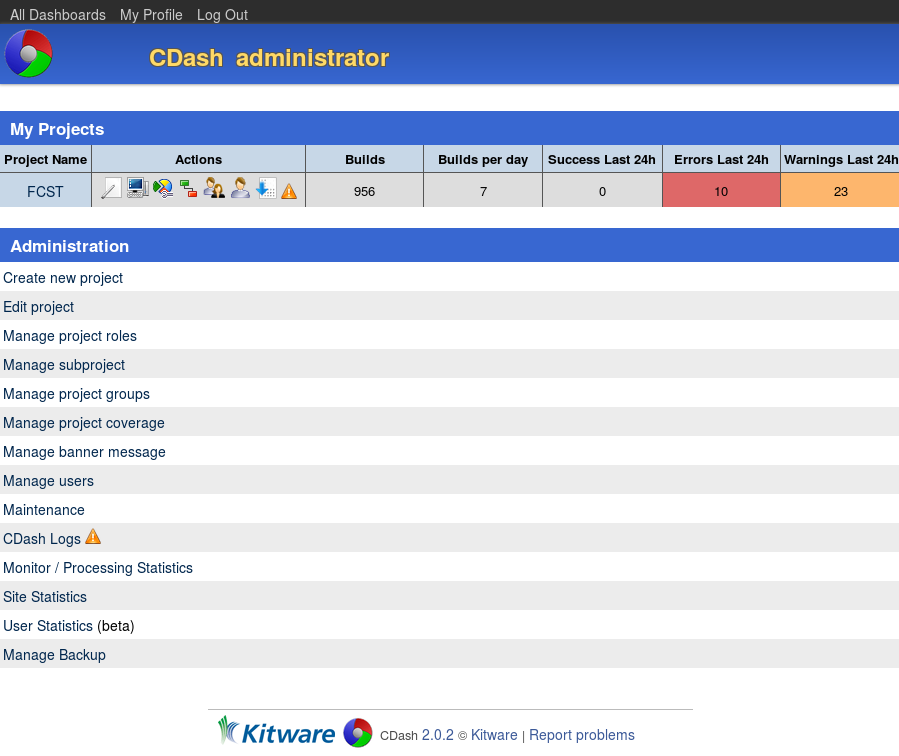
\includegraphics[width=1\textwidth]{figures/CDash/my_cdash.png}
\caption{''My CDash'' example page for an administrator}
\label{fig:my_cdash}
\end{figure}

Click on ''Manage users'', where new users can be added. Create the new user here and then go to the ''Project Roles'' page from the ''My CDash'' page. Here you can assign users to a project and also give their name repository name. CDash will use this during the testing process to email the users who last committed code if it crashes. The role of the user can also be assigned. The project administrator is in charge of the code and will always get emails if the code crashes or if there are errors in submitting results to the dashboard. Site maintainers are users of the code who also run and submit tests from their computers. They will be responsible for making sure that the code they are working on is running correctly and will be emailed if the tests they run are failing. This is achieved by having the user submit a test to the dashboard and then ''claiming the site''. CDash will keep a record of the 
computers that are performing tests and if a user claims a site they are responsible for the tests from that site. Normal users are users that simply use the code and want to keep track of code. 

Each user can have their own settings for how they are informed about the success of their tests. Going back to the ''My CDash'' page, under ''My Projects'' is a list of the dashboards the user is registered to. Under actions, the user can click the page icon to change their personal settings, such as email settings, role in a project and repository credential(s). Clicking the small computer icon will bring up a list of computers that have submitted tests to the dashboard, allowing the user to claim sites. 

There is one more useful section on the ''My CDash'' page for administrators, the ''CDash Logs''. If there are parts of the site that are not working, this is a useful place to look. It also logs other information such which users were emailed if a test has failed. 

\subsubsection{The CDash interface}

If the project has just been created, then project home page should now be available, with 5 lines saying ''no Nightly builds'' etc. This is the main page of the project, where all the information about the testing will be seen. It can be accessed by going to ''My CDash'' and choosing the dashboard from the ''My Projects'' section. An example is given on figure \ref{fig:project_page}.

\begin{figure}[!h]
\centering
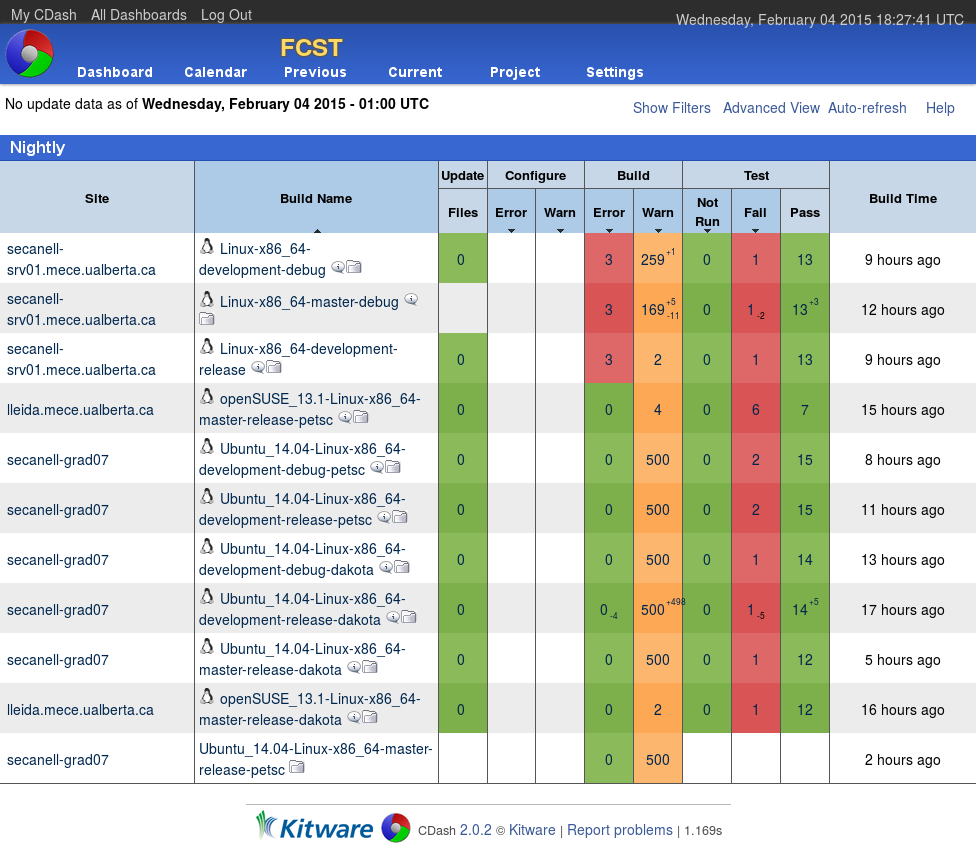
\includegraphics[width=1\textwidth]{figures/CDash/cdash.png}
\caption{Project's main page example}
\label{fig:project_page}
\end{figure}

On the project's main page, we can see the information given by CDash about test results for various builds and testing machines. From the dashboard, you know on which machine the tests were run (''Site''), what were the operating system and OpenFCST build parameters (''Build Name''), and detailed information on test results. A normal test run by CTest is to automatically update the code using \verb!git!, configure the code, build the code and then run tests to ensure that the code is behaving as expected.

In this test, performed on the 4th of February 2015, a testing sequence was run on three different machines, \verb!secanell-srv01.mece.ualberta.ca! (our main server; openSUSE~12.3), \verb!lleida.mece.ualberta.ca! (openSUSE~13.1), and \verb!secanell-grad07! (Ubuntu~14.04). If there are any locally modified files, CDash gives a warning in ''Configure'' section, and gives an error if there are conflicts. Usually, if the tests are being run on code that is located on the testing machine, there should not be any issues with the update process as nobody will be working on the code on those computers.

The ''Build'' section returns errors and warnings that appeared on the OpenFCST building stage. The ''Test'' section shows number of tests that were failed or passed. Each of the numbers shown can be clicked on to give more information. For example, if part of the build returns a warning as it did in the example above, clicking on the number will show the page given on figure \ref{fig:cdash_warning}.

\begin{figure}[!h]
\centering
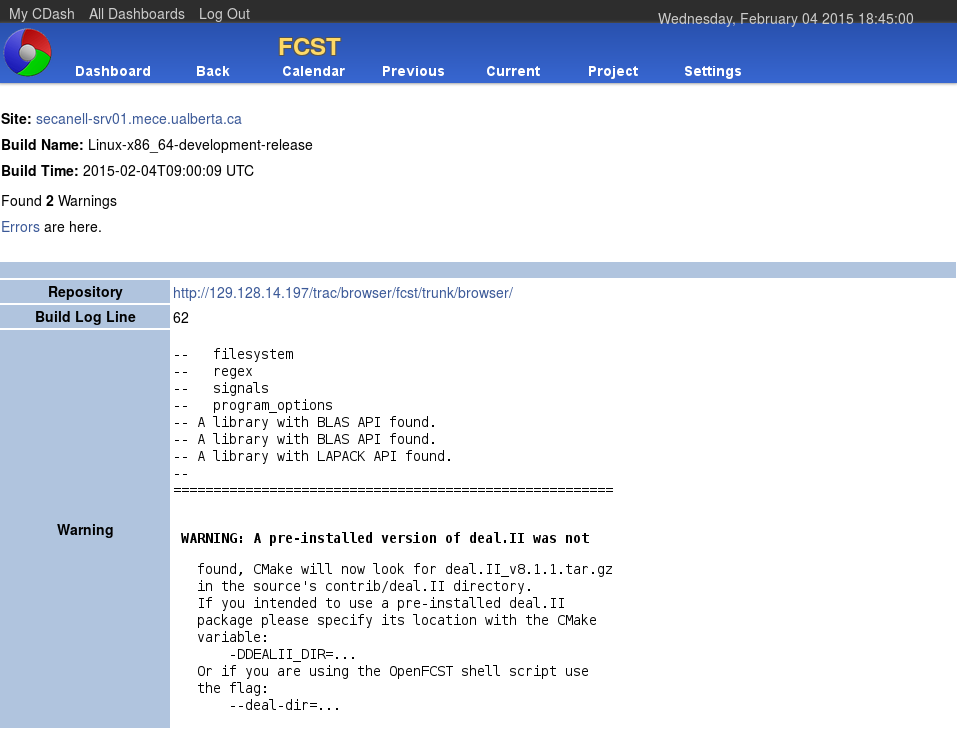
\includegraphics[width=1\textwidth]{figures/CDash/cdash_warning.png}
\caption{Example of the warning information page}
\label{fig:cdash_warning}
\end{figure}

\section{Configuring CTest}

\subsection{Testing your code in your local revision}
Before committing any changes made in your local revision, you should make sure that your working copy  passess provided tests. You can test your working copy of OpenFCST by typing the following in the command line in the OpenFCST main folder:
\begin{lstlisting}
$./run_tests
\end{lstlisting}

All test cases that have been programmed will be executed. Test summary output will be written to tests\_summary.log, and all OpenFCST output will be written to tests\_output.log. At present there are several tests provided, for various applications and the unit testing suite. 

\subsection{Setting up a CTest testing suite}\label{sec:setting_up_CTest}

When setting up a test using CTest, the normal procedure is to use the CMake suite of tools to configure and compile the code. Setting up CTest is then a very simple addition to this process.  To do this a ''steering'' file needs to be created, which will extract information about the computer and implement the commands for the update, configure, build and testing of the code. Setting up this file, called \verb!nightly_tests.cmake!, will be described by going through the file created for one of the testing machines, as well as its contributing files and associated processes.

To simply install a nightly test system on Linux, one can follow the following quick steps:
\begin{enumerate}
 \item Copy \verb!nightly_tests! \verb!.sh! and \verb!.cmake! to the OpenFCST root folder (where the install scripts reside).
 \item Edit the address line in that script to cd to OpenFCST root folder. Use the full address, e.g. \verb!/home/cdash/openfcst/!.
 \item Set up \verb!git! user credential caching as follows:
  \subitem Clear you credentials: \verb!git config credential.helper clear!
  \subitem Set the credentials to store: \verb!git config credential.helper store!
  \subitem Finally \verb!git pull! and enter your credentials
  \subitem More info at  \url{http://tinyurl.com/git-password}
\end{enumerate}

\subsubsection{The main steering file}

Two similar testing systems are supplied with OpenFCST. The \verb!run_tests! script will run test cases and report results directly back to the user. The nightly testing system is more thorough: it will update, build, install, and test the code for multiple branches and build modes, then finally report testing results to a CDash server which displays the results to other developers.

Here we will go through the nightly tests steering file, \verb!nightly_tests.cmake!, section by section.

\small \begin{lstlisting}
# -----------------------------------------------------------  
# -- Get environment
# -----------------------------------------------------------  

## -- Set hostname
## --------------------------
find_program(HOSTNAME_CMD NAMES hostname)
exec_program(${HOSTNAME_CMD} ARGS OUTPUT_VARIABLE HOSTNAME)

#Name of this computer
set(CTEST_SITE                          "${HOSTNAME}")

## -- Set site / build name
## --------------------------

find_program(UNAME NAMES uname)
macro(getuname name flag)
  exec_program("${UNAME}" ARGS "${flag}" OUTPUT_VARIABLE
                                               "${name}")
endmacro(getuname)

getuname(osname -s)
getuname(osrel  -r)
getuname(cpu    -m)


set(MODEL                               "Nightly")

## -- SVN command
## ----------------
find_program(CTEST_GIT_COMMAND NAMES git)

## -- make command
## -----------------
find_program(MAKE NAMES make)
\end{lstlisting}\normalsize

The first section, ''get environment'', contains commands that will find the name and some of the specifications of the computer, as well as the commands for the call to \verb!CMake! and \verb!git!. Here we also give the type of tests we are running. In this case we are running ''Nightly'' tests, so CDash will display the results from this build in the nightly section of the interface. Other choices are ''Continuous'' and ''Experimental''.

The file now gets specific to the tests that we are performing, e.g. defines a path to other CTest files (read on):

\small \begin{lstlisting}
# -----------------------------------------------------------  
# -- build specificFCST
# -----------------------------------------------------------  

## -- DashBoard Root
set(CTEST_DASHBOARD_ROOT        ${CMAKE_CURRENT_LIST_DIR})

## -- SRC Dir
set(CTEST_SOURCE_DIRECTORY     "${CTEST_DASHBOARD_ROOT}/
                                             Install/test")

## -- BIN Dir                                            
set(CTEST_BINARY_DIRECTORY     "${CTEST_SOURCE_DIRECTORY}/
                                build-${CTEST_BUILD_NAME}")
\end{lstlisting}\normalsize

Next, we set some directories. The root folder is OpenFCST root directory, where the install scripts, \verb!src/!, \verb!Install/! and \verb!Build/! folders exist. The source folder is where additional \verb!.cmake! files exist, as well as the individual test cases. The binary directory is where we will store the results from the test we are going to run. 

Pretty much all the following code does is setting an update command, defining a directory for CTest custom files (later in this manual).

\small \begin{lstlisting}
# -----------------------------------------------------------  
# -- commands
# -----------------------------------------------------------  

## -- Update Command
set(CTEST_UPDATE_COMMAND        "${CTEST_GIT_COMMAND}")

# -----------------------------------------------------------  
# -- Configure CTest
# -----------------------------------------------------------  

## -- read CTestCustom.cmake file
ctest_read_custom_files("${CTEST_SOURCE_DIRECTORY}")

# -----------------------------------------------------------  
# -- Settings
# -----------------------------------------------------------  

## -- Process timeout in seconds
set(CTEST_TEST_TIMEOUT           "14400")

## -- Set output to english
set( $ENV{LC_MESSAGES}      "en_EN" )

\end{lstlisting}\normalsize

Then, we specify Bitbucket branches of OpenFCST that we are going to test, build modes, build flags, and the name of the operating system. Note that \verb!osname! variable that we declared earlier does not contain Linux distribution name and its version, e.g. ''openSUSE 13.1'' or ''Ubuntu 14.04''. On each testing machine, you need to modify \verb!DISTR_NAME! declaration line in this file.

\small \begin{lstlisting}
# -----------------------------------------------------------  
# -- Run CTest
# -----------------------------------------------------------  

##----Remove comments made using a single hash key in order
##----to get CTest to test that component.

 ############################################################
 #####################                  #####################
 ##################### Testing sequence #####################
 #####################                  #####################
 ############################################################ 

 set(GIT_BRANCHES "development" "master")
 set(BUILD_MODES "release" "debug")
 set(BUILD_FLAGS "dakota" "petsc")
 set(DISTR_NAME "openSUSE_13.1")

\end{lstlisting}\normalsize

After that, we create a file (rewrite if it exists) \verb!config.txt! in \verb!/Install/test! that contains certain flags. You will see later that another \verb!.cmake! file, specifically \verb!CTestTestfile.cmake!, reads this text file and enables/disables some of the test cases depending on what flag was written to \verb!config.txt!.

\small \begin{lstlisting}
 ## WRITE: -- First, turn all options off.

 file(WRITE ${CTEST_DASHBOARD_ROOT}/Install/test/config.txt
                       "List of current build flags:" "\n")
 file(APPEND ${CTEST_DASHBOARD_ROOT}/Install/test/config.txt
                    "PETScOFF" "\n") # Turn PETSc option off
 file(APPEND ${CTEST_DASHBOARD_ROOT}/Install/test/config.txt
                  "DAKOTAOFF" "\n") # Turn Dakota option off

 ## WRITE: -- End
\end{lstlisting}\normalsize

Finally, in several \verb!FOREACH! loops, we ckeckout branches (update local files), build OpenFCST, run tests, and submit the results to CDash. In this example, we test the following builds:

\begin{itemize}
\item master-release-dakota;
\item master-release-petsc;
\item development-release-dakota;
\item development-release-petsc;
\item development-debug-dakota;
\item development-debug-petsc,
\end{itemize}

\noindent which correspond to 

\begin{itemize}
\item OpenFCST version from ''master'' branch compiled in ''release'' mode with \verb!--with-dakota! flag;
\item OpenFCST version from ''master'' branch compiled in ''release'' mode with \verb!--with-petsc! flag;
\item OpenFCST version from ''development'' branch compiled in ''release'' mode with \verb!--with-dakota! flag;
\item OpenFCST version from ''development'' branch compiled in ''release'' mode with \verb!--with-petsc! flag;
\item OpenFCST version from ''development'' branch compiled in ''debug'' mode with \verb!--with-dakota! flag;
\item OpenFCST version from ''development'' branch compiled in ''debug'' mode with \verb!--with-petsc! flag.
\end{itemize}

For each build, we rewrite \verb!config.txt! to turn on/off Dakota- and PETSc-specific tests.

You might want to change the number of cores used for building OpenFCST depending on specifications of your machine. To do that, modify \verb!--cores! value in each of  \verb!set(CTEST_BUILD_COMMAND ...)! lines.

\small \begin{lstlisting}
 FOREACH(GIT_BRANCH ${GIT_BRANCHES})

 FOREACH(BUILD_FLAG ${BUILD_FLAGS})

  IF(GIT_BRANCH STREQUAL "master")

   set(BUILD_MODE "release")

   IF(BUILD_FLAG STREQUAL "dakota")
   
    file(WRITE
    ${CTEST_DASHBOARD_ROOT}/Install/test/config.txt
    "List of current build flags:" "\n")
    
    file(APPEND
    ${CTEST_DASHBOARD_ROOT}/Install/test/config.txt
    "PETScOFF" "\n")
    
    file(APPEND
    ${CTEST_DASHBOARD_ROOT}/Install/test/config.txt
    "DAKOTAON" "\n")
     
    set(CTEST_BUILD_COMMAND "./openFCST_install --cores=4
                                          --with-dakota")
                                          
   ELSEIF(BUILD_FLAG STREQUAL "petsc")
   
    file(WRITE
    ${CTEST_DASHBOARD_ROOT}/Install/test/config.txt
    "List of current build flags:" "\n")
    
    file(APPEND
    ${CTEST_DASHBOARD_ROOT}/Install/test/config.txt
    "PETScON" "\n")
    
    file(APPEND
    ${CTEST_DASHBOARD_ROOT}/Install/test/config.txt
    "DAKOTAOFF" "\n")
    
    set(CTEST_BUILD_COMMAND "./openFCST_install --cores=4
                                           --with-petsc")
                                           
   ENDIF()

    ## -- Checkout the branch
    execute_process (COMMAND ${CTEST_GIT_COMMAND} checkout
                                            ${GIT_BRANCH})
    set(CTEST_BUILD_NAME
    "${DISTR_NAME}-${osname}-${cpu}-${GIT_BRANCH}-
                             ${BUILD_MODE}-${BUILD_FLAG}")

    message(" -- Start dashboard ${MODEL} - ${GIT_BRANCH}
    - ${CTEST_BUILD_NAME} - ${BUILD_MODE} - ${BUILD_FLAG}
                                                     --")
                                                       
    ctest_start(${MODEL} TRACK ${MODEL})

    ## -- Update
    message(" -- Update ${MODEL} - ${GIT_BRANCH}
    - ${CTEST_BUILD_NAME} - ${BUILD_MODE}
                             -${BUILD_FLAG} --")
    ctest_update(
    SOURCE "${CTEST_DASHBOARD_ROOT}" RETURN_VALUE res)

    # -- BUILD, build the whole project
    message(" -- Build ${MODEL} - ${GIT_BRANCH}
    - ${CTEST_BUILD_NAME} - ${BUILD_MODE} -${BUILD_FLAG}
                                                    --")
    ctest_build(    BUILD  "${CTEST_DASHBOARD_ROOT}"
                                   RETURN_VALUE res)

    ## -- TEST
    message(" -- Test ${MODEL} - ${GIT_BRANCH}
    - ${CTEST_BUILD_NAME} -${BUILD_MODE} -${BUILD_FLAG}
                                                   --")
    ctest_test(     BUILD  "${CTEST_SOURCE_DIRECTORY}"
                                      RETURN_VALUE res)

    ## -- SUBMIT
    message(" -- Submit ${MODEL} - ${GIT_BRANCH}
    - ${CTEST_BUILD_NAME} -${BUILD_MODE} -${BUILD_FLAG}
                                                   --")
    ctest_submit(                     RETURN_VALUE res)

    message(" -- Finished ${MODEL}  - ${GIT_BRANCH}
    - ${CTEST_BUILD_NAME} -${BUILD_MODE} -${BUILD_FLAG}
                                                   --")

   ELSEIF(GIT_BRANCH STREQUAL "development")

    FOREACH(BUILD_MODE ${BUILD_MODES})

     IF(BUILD_FLAG STREQUAL "dakota")

      file(WRITE
      ${CTEST_DASHBOARD_ROOT}/Install/test/config.txt
                 "List of current build flags:" "\n")
                 
      file(APPEND
      ${CTEST_DASHBOARD_ROOT}/Install/test/config.txt
                                     "PETScOFF" "\n")   
                                        
      file(APPEND
      ${CTEST_DASHBOARD_ROOT}/Install/test/config.txt
                                     "DAKOTAON" "\n")
                                     

        IF(BUILD_MODE STREQUAL "release")
         set(CTEST_BUILD_COMMAND  "./openFCST_install
                           --cores=4  --with-dakota")
        ELSEIF(BUILD_MODE STREQUAL "debug")
         set(CTEST_BUILD_COMMAND  "./openFCST_install
          --cores=4  --with-dakota --openfcst-debug")
        ENDIF()

       ELSEIF(BUILD_FLAG STREQUAL "petsc")

        file(WRITE
        ${CTEST_DASHBOARD_ROOT}/Install/test/config.txt
                   "List of current build flags:" "\n")
                   
        file(APPEND
        ${CTEST_DASHBOARD_ROOT}/Install/test/config.txt
                                        "PETScON" "\n")
        file(APPEND
        ${CTEST_DASHBOARD_ROOT}/Install/test/config.txt
                                      "DAKOTAOFF" "\n")

        IF(BUILD_MODE STREQUAL "release")
          set(CTEST_BUILD_COMMAND  "./openFCST_install
                             --cores=4  --with-petsc")
        ELSEIF(BUILD_MODE STREQUAL "debug")
          set(CTEST_BUILD_COMMAND   "./openFCST_install
             --cores=4  --with-petsc --openfcst-debug")
        ENDIF()

       ENDIF()

       ## -- Checkout the branch
       execute_process (COMMAND ${CTEST_GIT_COMMAND} checkout
                                               ${GIT_BRANCH})
       set(CTEST_BUILD_NAME
       "${DISTR_NAME}-${osname}-${cpu}-${GIT_BRANCH}-
                                ${BUILD_MODE}-${BUILD_FLAG}")

       message(" -- Start dashboard ${MODEL} - ${GIT_BRANCH}
       - ${CTEST_BUILD_NAME} - ${BUILD_MODE} - ${BUILD_FLAG}
                                                     --")
                                                       
       ctest_start(${MODEL} TRACK ${MODEL})

       ## -- Update
       message(" -- Update ${MODEL} - ${GIT_BRANCH}
       - ${CTEST_BUILD_NAME} - ${BUILD_MODE}
                                -${BUILD_FLAG} --")
       ctest_update(
       SOURCE "${CTEST_DASHBOARD_ROOT}" RETURN_VALUE res)

       # -- BUILD, build the whole project
       message(" -- Build ${MODEL} - ${GIT_BRANCH}
       - ${CTEST_BUILD_NAME} - ${BUILD_MODE} -${BUILD_FLAG}
                                                       --")
      ctest_build(    BUILD  "${CTEST_DASHBOARD_ROOT}"
                                      RETURN_VALUE res)
 
       ## -- TEST
       message(" -- Test ${MODEL} - ${GIT_BRANCH}
       - ${CTEST_BUILD_NAME} -${BUILD_MODE} -${BUILD_FLAG}
                                                      --")
       ctest_test(     BUILD  "${CTEST_SOURCE_DIRECTORY}"
                                         RETURN_VALUE res)

       ## -- SUBMIT
       message(" -- Submit ${MODEL} - ${GIT_BRANCH}
       - ${CTEST_BUILD_NAME} -${BUILD_MODE} -${BUILD_FLAG}
                                                      --")
       ctest_submit(                     RETURN_VALUE res)

       message(" -- Finished ${MODEL}  - ${GIT_BRANCH}
       - ${CTEST_BUILD_NAME} -${BUILD_MODE} -${BUILD_FLAG}
                                                      --")

     ENDFOREACH()
   ENDIF()

 ENDFOREACH() # BUILD_FLAG

    file(WRITE
    ${CTEST_DASHBOARD_ROOT}/Install/test/config.txt
               "List of current build flags:" "\n")
    
    file(APPEND
    ${CTEST_DASHBOARD_ROOT}/Install/test/config.txt
                                   "PETScOFF" "\n")
                                   
    file(APPEND
    ${CTEST_DASHBOARD_ROOT}/Install/test/config.txt
                                  "DAKOTAOFF" "\n")

 ENDFOREACH() # GIT_BRANCH
\end{lstlisting}\normalsize

This completes the steering file.

Note that the test command was not specified in the steering file. This is actually done in another file which will be discussed next.

\subsubsection{Contributing files}

There are three contributing files that are needed by CTest. Information on the three files can be found at the following page:
\url{http://www.vtk.org/Wiki/CTest:Using_CTEST_and_CDASH_without_CMAKE}.

The first is the \verb!CTestCustom.cmake! file that is used to customize the testing process:

\small \begin{lstlisting}
set(CTEST_CUSTOM_MAXIMUM_NUMBER_OF_WARNINGS "500" )
set(CTEST_CUSTOM_MAXIMUM_FAILED_TEST_OUTPUT_SIZE "100000" )
set(CTEST_CUSTOM_MAXIMUM_PASSED_TEST_OUTPUT_SIZE "100000" )
\end{lstlisting}\normalsize

Here we limit the number of warnings that CTest will report and we also limit the size of the output of the results file. More options are given on the webpage mentioned above.

The next file is the \verb!CTestConfig.cmake! file which gives CTest the information about the CDash website:

\small \begin{lstlisting}
set(CTEST_PROJECT_NAME "FCST")
set(CTEST_NIGHTLY_START_TIME "01:00:00 UTC")

set(CTEST_DROP_METHOD "http")
set(CTEST_DROP_SITE "129.128.14.197")
set(CTEST_DROP_LOCATION "/CDash/submit.php?project=FCST")
set(CTEST_DROP_SITE_CDASH TRUE)
\end{lstlisting}\normalsize

Note that the time set is just a time stamp for CDash. The actual time when tests are run is set using Cron (read on).

The last CTest file is \verb!CTestTestfile.cmake!. This is where we specify the tests we want to run. This is done using the following command:

\small \begin{lstlisting}
ADD_TEST(app_cathode "test_cases/app_cathode_case.sh")
\end{lstlisting}\normalsize

All the tests are added with a simple command like that one.

The command contains the name of the test, \verb!app_cathode!, and the test file to be executed. Note that the test file is a bash script that actually runs the code. This script will run the code and then compare the results to the expected results file:

\small \begin{lstlisting}
cd ../data/cathode/testing
rm polarization_curve.dat
../../../bin/fuel_cell-2d.bin main_app_cathode_test.prm

if [ "${PIPESTATUS[0]}" != "0" ]; then
	echo  2>&1 | tee tests_summary.log
	echo  "Results summary from the app_cathode test:"
	             2>&1 | tee --append tests_summary.log
	echo  2>&1 | tee --append tests_summary.log
	echo "-----" 2>&1 | tee --append tests_summary.log
	echo "The simulation did not run correctly. Please
	review the tests_output.log file  "  2>&1 | tee
	                        --append tests_summary.log
	echo "-----" 2>&1 | tee --append tests_summary.log
	echo  2>&1 | tee --append tests_summary.log
	cat tests_summary.log >> ../../../tests_summary.log 
  exit 2
else
	../../../test/csvPoleCurveCompare.py
	            polarization_curve.dat test_results.dat
	if [ "${PIPESTATUS[0]}" != "0" ]; then
		echo  2>&1 | tee tests_summary.log
		echo  "Results summary from the app_cathode
		test:" 2>&1 | tee --append
		                          tests_summary.log
		echo 2>&1 | tee --append
		                          tests_summary.log
		echo "--" 2>&1 | tee --append
		                          tests_summary.log
		echo "Results from the test do not match
		expected results" 2>&1 | tee --append
		                          tests_summary.log
		echo "Please check the results in
		polarization_curve.dat against that of
		test_results.dat" 2>&1 | tee --append
		                          tests_summary.log
		echo "--" 2>&1 | tee --append
		                          tests_summary.log
		echo 2>&1 | tee --append
		                          tests_summary.log
		cat tests_summary.log >>
		                 ../../../tests_summary.log 
		exit 2
	else 
		echo  2>&1 | tee tests_summary.log
		echo  "Results summary from the app_cathode
		   test:" 2>&1 | tee --append
		                          tests_summary.log
		echo 2>&1 | tee --append tests_summary.log
		echo "--" 2>&1 | tee --append
		                          tests_summary.log
		echo "Results from the test match expected
		 results" 2>&1 | tee --append
		                          tests_summary.log
		echo  "-" 2>&1 | tee --append
		                          tests_summary.log
		echo 2>&1 | tee --append tests_summary.log
		cat tests_summary.log >>
		                 ../../../tests_summary.log 
		exit 0
	fi
fi
\end{lstlisting}\normalsize

The test case will run the code with the \verb!app_cathode! test case file. If anything goes wrong, the script will save error information to \verb!tests_summary.log! file.

It is worth to note how \verb!CTestTestfile.cmake! interacts with \verb!config.txt! file that we mentioned when we were discussing the steering file.

The \verb!CTestTestfile.cmake! version located in \verb!src/! folder of OpenFCST contains the following line:

\small \begin{lstlisting}
file(STRINGS @CMAKE_INSTALL_PREFIX@/test/config.txt FLAGS)
\end{lstlisting}\normalsize

When OpenFCST is being installed, it replaces \verb!@CMAKE_INSTALL_PREFIX@! with actual path to \verb!Install/! directory. Note that, after the installation process, you will have two sets of CTest configuration files: in \verb!Install/! folder and in \verb!src/! folder. The tests are run in \verb!Install/! folder.

All lines from \verb!config.txt! are read to the \verb!FLAGS! string list variable. Then, the commands

\small \begin{lstlisting}
list(FIND FLAGS "PETScON" PETSc_FLAG)
list(FIND FLAGS "DAKOTAON" Dakota_FLAG)
\end{lstlisting}\normalsize

\noindent check if certain flags were set on. In general, \verb!list(FIND list value variable)! returns index of the element in the \verb!list! through \verb!variable! if the \verb!value! was found or -1 if it was not. So we use this fact to enable/disable our package-specific tests like those which need PETSc or Dakota:

\small \begin{lstlisting}
## -- Parallel tests
IF(PETSc_FLAG GREATER -1)
  ADD_TEST(app_cathode_parallel
                 "test_cases/app_cathode_parallel_case.sh")
  ADD_TEST(app_diffusion_3D_parallel
                 "test_cases/app_diffusion_3D_parallel.sh")
ENDIF() # PETSc_FLAG

# -- Dakota integration test:
IF(Dakota_FLAG GREATER -1)
  ADD_TEST(dakota_parametric
                   "test_cases/app_cathode_dakota_case.sh")
ENDIF() # Dakota_FLAG
\end{lstlisting}\normalsize

\subsubsection{Setting an automatic nightly testing}

To make the tests run every night, cron is used. Cron is a program that allows a user to schedule programs to run at a set time automatically. The script and time and day it should be run at are specified in a file created by cron. The bash script we use is called \verb!nightly_tests.sh! and it is packaged in a zip file inside the \verb!test/! folder. The script sets some environment variables required to build OpenFCST, cleans OpenFCST and its contribs, and then launches the CTest steering file. After unpacking files from the archive as it was described in subsection \ref{sec:setting_up_CTest},  add a \verb!Cron! job to execute \verb!nightly_tests.sh! nightly. Use \verb!crontab -e!. The line you add should look like this:\\

\verb!0 02 * * * /bin/bash /home/cdash/openfcst/nightly_tests.sh!\\
 
The address of the script has to be full.

This cron job will run \verb!nightly_tests.sh! every night at 2 a.m. local time. For more info on how to configure Cron jobs, go to \url{http://tinyurl.com/crontab-howto}.

This completes the setup of the testing suite.

%%===============================================================
%%===============================================================
%%===============================================================
%%===============================================================
%%===============================================================
%%===============================================================